\section*{Kapitel 3 - Quadratsummenzerlegung und statistische Inferenz im multiplen linearen Regressionsmodell}

\begin{multicols*}{3}

\tikzstyle{mybox} = [draw=black, fill=white, very thick,
    rectangle, rounded corners, inner sep=10pt, inner ysep=10pt]
\tikzstyle{fancytitle} =[fill=black, text=white, font=\bfseries]



%------------ Quadratsummenzerlegung ---------------
\begin{tikzpicture}
    \node [mybox] (box){%
        \begin{minipage}{0.3\textwidth}
        Gegeben sei das multiple lineare Regressionsmodell mit
        $\rang(\bX) = p'$. Dann gilt
        \footnotesize{
        $$
        \underbrace{(\bY - \bar\bY)^\top (\bY - \bar\bY)}_{SST} =
        \underbrace{(\bY - \hbY)^\top (\bY - \hbY)}_{SSE} + 
        \underbrace{(\hbY - \bar\bY)^\top (\hbY - \bar\bY)}_{SSM}.
        $$}

        \begin{align*}
        & \text{SST(otal):} & & \text{Gesamt-Quadratsumme (korrigiert)}\\
        & \text{SSE(rror):} & &\text{Fehler-Quadratsumme}\\
        & \text{SSM(odel):} & &\text{Modell-Quadratsumme}\\
        \end{align*}
        \end{minipage}
    };
%------------ Quadratsummenzerlegung Header ---------------------
\node[fill = purple, text=white, font=\bfseries, right=10pt] at (box.north west) {Quadratsummenzerlegung};
\end{tikzpicture}


%------------ Quadratsummenzerlegung ohne b0 ---------------
\begin{tikzpicture}
    \node [mybox] (box){%
        \begin{minipage}{0.3\textwidth}
        Gegeben sei das multiple lineare Regressionsmodell mit, aber ohne Absolutglied $\gb0$. Dann gilt
        \footnotesize{
        $$
        \underbrace{\bY^\top \bY}_{SST^*} =
        \underbrace{(\bY - \hbY)^\top (\bY - \hbY)}_{SSE} + 
        \underbrace{\hbY^\top \hbY}_{SSM^*}.
        $$}

        \begin{align*}
        & \text{$SST^*$:} & & \text{Gesamt-Quadratsumme (nicht korrigiert)}\\
        & \text{$SSE$:} & &\text{Fehler-Quadratsumme (wie zuvor)}\\
        & \text{$SSM^*$:} & &\text{Modell-Quadratsumme (nicht korrigiert)}\\
        \end{align*}
        \end{minipage}
    };
%------------ Quadratsummenzerlegung ohne b0 Header ---------------------
\node[fill = purple, text=white, font=\bfseries, right=10pt] at (box.north west) 
{Quadratsummenzerlegung ohne $\beta_0$};
\end{tikzpicture}


%------------ Erwartungswerte der Quadratsummen ---------------
\begin{tikzpicture}
    \node [mybox] (box){%
        \begin{minipage}{0.3\textwidth}
        Gegeben sei das multiple lineare Regressionsmodell mit den üblichen Annahmen. 
        Wir definieren
        $$\be = \begin{pmatrix}
            1 \\ \vdots \\ 1
        \end{pmatrix}  \text{ und } \bP_{\be} = \be(\be^\top \be)^{-1}\be^\top \text{ und } \bQ_{\be} = \bI - \bP_{\be}.$$
        Dann gilt
        \begin{align*}
        & \bP_{\be}\bY = \bar\bY && \quad { und } \quad \bQ_{\be}\bY = \bY - \bar\bY \\
        & \E(SST^*) &&= \ssd n + \bbeta^\top \bX^\top \bX \bbeta \\
        & \E(SST) &&= \ssd (n-1) + \bbeta^\top (\bQ_{\be}\bX)^\top (\bQ_{\be}\bX) \bbeta \\
        & \E(SSE) &&= \ssd (n-p') \\
        & \E(SSM^*) &&= \ssd p' + \bbeta^\top \bX^\top \bX \bbeta \\
        & \E(SSM) &&= \ssd (p'-1) + \bbeta^\top (\bQ_{\be}\bX)^\top (\bQ_{\be}\bX) \bbeta
        \end{align*}
        Wir können diese Eigenschaften zur Konstruktion von Tests verwenden.
        Es gilt nämlich unter anderem
        $\bbeta = 0 \implies \E(SST^*) = \ssd n$\\
        $\gb{1} = \dots = \gb{p} = 0 \implies \E(SSM) = \ssd (p'-1)$
        \end{minipage}
    };
%------------ Erwartungswerte der Quadratsummen Header ---------------------
\node[fill = purple, text=white, font=\bfseries, right=10pt] at (box.north west) 
{Erwartungswerte der Quadratsummen};
\end{tikzpicture}

%------------ Mittlere Quadratsummen ---------------
\begin{tikzpicture}
    \node [mybox] (box){%
        \begin{minipage}{0.3\textwidth}
        Wir definieren entsprechend der Zahl der Freiheitsgrade die
        \tc{mittleren Quadratsummen} als
        \begin{align*}
            &\text{MSE} = \frac{SSE}{n-p'} = \hssd \\
            &\text{MSM} = \frac{SSM}{p'-1} \\
            &\text{MST} = \frac{SST}{n-1} \\
            &\text{MSM}^* = \frac{SSM^*}{p'} \\
            &\text{MST}^* = \frac{SST^*}{n}
        \end{align*}

        \end{minipage}
    };
%------------ Mittlere Quadratsummen Header ---------------------
\node[fill = purple, text=white, font=\bfseries, right=10pt] at (box.north west) 
{Mittlere Quadratsummen};
\end{tikzpicture}

%------------ R^2 ---------------
\begin{tikzpicture}
    \node [mybox] (box){%
        \begin{minipage}{0.3\textwidth}
        Gegeben sei das multiple lineare Regressionsmodell mit allen Annahmen.
        Dann definieren wir das \tc{Bestimmtheitsmaß} $R^2$ als
        $$R^2 = \frac{SSM}{SST} = 1 - \frac{SSE}{SST} = r_{\bY \hbY}^2 \in [0,1]$$
        wobei $r_{\bY \hbY}$ der Korrelationskoeffizient zwischen $\bY$ und $\hbY$ ist.

        Wir interpretieren $R^2$ als den Anteil der Varianz von $\bY$, die durch
        das Modell erklärt wird. Ein hohes $R^2$ deutet darauf hin, dass wir
        unser Modell gut nutzen können, um $\bY$ zu erklären. $R^2$ steigt mit
        steigender Anzahl an Kovariablen, auch wenn diese kaum/keine
        Erklärungskraft haben. Es ist daher nicht sinnvoll, $R^2$ zwischen
        Modellen zu vergleichen, die unterschiedlich viele Kovariablen haben.
        Hierfür nutzen wir das
        \tc{adjustierten Bestimmtheitsmaß} 
        \begin{align*}
            R_{\text{adj}}^2 &= \frac{MSM}{MST} = 1 - \frac{MSE}{MST} = 1 -
        \frac{SSE/(n-1)}{SST/(n-p')} \\
        & = 1 - \frac{n-1}{n-p'}(1 - R^2)
        \end{align*}
        Für $n \gg p'$ gilt $R_{\text{adj}}^2 \approx R^2$.\\
        \tc{!} Bei einem Modell ohne Absolutglied ist $R^2$ nach obiger Definition
        nicht sinnvoll, da es dann auch negative Werte annehmen kann. Das kommt daher, dass
        die Zerlegung $SST = SSE + SSM$ nicht mehr gilt.
        Stattdessen ist es sinnvoll, $R^2$ als $\frac{SSM^*}{SST^*} = 1 - \frac{SSE}{SST^*}$ zu definieren.

        

        \end{minipage}
    };
%------------ R^2 Header ---------------------
\node[fill = black, text=white, font=\bfseries, right=10pt] at (box.north west) 
{$R^2$};
\end{tikzpicture}

%------------ Multivariate Normalverteilung ---------------
\begin{tikzpicture}
    \node [mybox] (box){%
        \begin{minipage}{0.3\textwidth}
        Eine Zufallsvariable $\bZ \in \R^n$ heißt \tc{multivariat
        normalverteilt} mit Erwartungswert $\bmu \in \R^n$ und positiv definiter
        Kovarianzmatrix $\Sigma \in \R^{n \times n}$, wenn ihre Dichte gegeben
        ist durch
        $$f(\bz) = \frac{1}{(2\pi)^{n/2}|\Sigma|^{1/2}}
        \exp\left(-\frac{1}{2}(\bz - \bmu)^\top \Sigma^{-1}(\bz -
        \bmu)\right).$$
        Wir schreiben $\bZ \sim \Ncal_n(\bmu, \Sigma)$.

        \end{minipage}
    };
%------------ Multivariate Normalverteilung Header ---------------------
\node[fill = black, text=white, font=\bfseries, right=10pt] at (box.north west) 
{Multivariate Normalverteilung};
\end{tikzpicture}

%------------ Multivariate Normalverteilung Eigenschaften ---------------
\begin{tikzpicture}
    \node [mybox] (box){%
        \begin{minipage}{0.3\textwidth}
        Sei $\bZ \sim \Ncal_n(\bmu, \Sigma)$ und $\bA \in \R^{m \times n}$ mit $\rang(\bA) = m$. Dann gilt
        \begin{enumerate}
            \item $\E(\bZ) = \bmu$
            \item $\V(\bZ) = \Sigma$
            \item $\bA\bZ \sim \Ncal_m(\bA\bmu, \bA\Sigma\bA^\top)$
            \item Es existiert eine orthogonale Matrix $\bT \in \R^{n \times n}$ mit
            $\bT \Sigma \bT^\top = \diag(\lambda_1, \dots, \lambda_n)$, so dass
            $$\bT\bZ \sim \Ncal_n(\bT\bmu, \diag(\lambda_1, \dots, \lambda_n))$$
        \end{enumerate}
        

        \end{minipage}
    };
%------------ Multivariate Normalverteilung Eigenschaften Header ---------------------
\node[fill = purple, text=white, font=\bfseries, right=10pt] at (box.north west) 
{Eigenschaften von $\Ncal_n(\bmu, \Sigma)$};
\end{tikzpicture}
    

%------------ Chi-Quadrat Verteilung ---------------
\begin{tikzpicture}
    \node [mybox] (box){%
        \begin{minipage}{0.3\textwidth}
        Sei $\bZ \sim \Ncal_n(\bmu, \bI)$, so heißt $\bW = \bZ^\top\bZ = \sumin Z_i^2$ (nicht-zentral) \tc{Chi-Quadrat-verteilt} und wir schreiben
        $$W \sim \chi^2(n, \delta).$$
        Wir nennen $n$ die \tc{Zahl der Freiheitsgrade} und $\delta = \bmu^\top\bmu$ den \tc{Nicht-Zentralitätsparameter}. 
        Es gilt
        \begin{align*}
            \E(W) &= n + \delta \\
            \V(W) &= 2n + 4\delta \\
        \end{align*}

        \end{minipage}
    };
%------------ Chi-Quadrat Verteilung Header ---------------------
\node[fill = black, text=white, font=\bfseries, right=10pt] at (box.north west) 
{Chi-Quadrat Verteilung};
\end{tikzpicture}

%------------ t-Verteilung ---------------
\begin{tikzpicture}
    \node [mybox] (box){%
        \begin{minipage}{0.3\textwidth}
        Seien $Z \sim \Ncal(\delta, 1)$ und $W \sim \chi^2(n, 0)$ unabhängig.
        Dann heißt $T = \frac{Z}{\sqrt{\frac{W}{n}}}$ (nicht-zentral) \tc{t-verteilt} mit $n$ \tc{Freiheitsgraden} und \tc{Nicht-Zentralitätsparameter} $\delta$ 
        und wir schreiben $$T \sim t(n, \delta).$$
        Es gilt
        $$\E(T) = \delta \sqrt{\frac{n}{2}} \frac{\Gamma(\frac{n-1}{2})}{\Gamma(\frac{n}{2})} \text{ für } n > 1$$
        \end{minipage}
    };
%------------ t-Verteilung Header ---------------------
\node[fill = black, text=white, font=\bfseries, right=10pt] at (box.north west) 
{t-Verteilung};
\end{tikzpicture}

%------------ F-Verteilung ---------------
\begin{tikzpicture}
    \node [mybox] (box){%
        \begin{minipage}{0.3\textwidth}
        Sei $W_1 \sim \chi^2(n_1, \delta)$ und $W_2 \sim \chi^2(n_2, 0)$ unabhängig.
        Dann heißt $X =  \frac{W_1/n_1}{W_2/n_2}$ (nicht-zentral) \tc{F-verteilt} mit $n_1$ und $n_2$ \tc{Freiheitsgraden} und \tc{Nicht-Zentralitätsparameter} $\delta$
        und wir schreiben $$X \sim F(n_1, n_2, \delta).$$
        Es gilt
        $$\E(X) = \frac{n_2 + \frac{n_2\delta}{n_1}}{n_2 - 2} \text{ für } n_2 > 2$$
        \end{minipage}
    };
%------------ F-Verteilung Header ---------------------
\node[fill = black, text=white, font=\bfseries, right=10pt] at (box.north west) 
{F-Verteilung};
\end{tikzpicture}

%------------ Satz von Cochran ---------------
\begin{tikzpicture}
    \node [mybox] (box){%
        \begin{minipage}{0.3\textwidth}
        Sei 
        \begin{itemize}
            \item $\bZ \sim \Ncal_n(\bmu, \Sigma)$,
            \item $\bA \in \R^{n \times n}$ mit $\rang(\bA) = r$ und $\bA^2 = \bA$,
            \item $\bB \in \R^{n \times n}$ mit $\bB^2 = \bB$ und $\bB^\top = \bB$,
            \item $\bC \in \R^{m \times n}$.
        \end{itemize}
        dann gilt
        \begin{align*}
            &\bZ^\top\bA\bZ \sim \chi^2(r, \bmu^\top\bA\bmu) \\
            &\bC\bA = \mathbf{0} \implies \bC\bZ \text{ und } \bZ^\top\bA\bZ \text{ sind unabhängig.}\\
            &\bA\bB = \mathbf{0} \implies \bZ^\top\bA\bZ \text{ und } \bZ^\top\bB\bZ \text{ sind unabhängig.}
        \end{align*}


        \end{minipage}
    };
%------------ Satz von Cochran Header ---------------------
\node[fill = purple, text=white, font=\bfseries, right=10pt] at (box.north west) 
{Satz von Cochran};
\end{tikzpicture}

%------------ Verteilung des KQ-Schätzers ---------------
\begin{tikzpicture}
    \node [mybox] (box){%
        \begin{minipage}{0.3\textwidth}
        Gegeben sei das multiple lineare Regressionsmodell mit $\rang(\bX) = p'$
        und den üblichen Annahmen über $\beps$. Dann gilt für den KQ-Schätzer
        $\hbbeta$:
        
        \begin{align*}
            \hbbeta &\sim \Ncal_p(\bbeta, \ssd(\bX^\top\bX)^{-1}) \\
            \hat{\Sigma}_{\hbbeta} &:= \hssd (\bX^\top\bX)^{-1} \\
            (n-p')\frac{\hssd}{\ssd} &\sim \chi^2(n-p') \\
            \hssd \text{ und } \hbbeta &\text{ sind unabhängig.} \\
            \hssd_{\hbe{k}} &:= (\hat{\Sigma}_{\hbbeta})_{kk} \\
            \frac{\hbe{k} - \beta_{k}}{\sqrt{\hssd_{\hbe{k}}}} &\sim t(n-p', 0)
        \end{align*}

        Um exakte Tests durchzuführen, ist die Normalverteilungsannahme für $\beps$ notwendig.
        Jedoch gelten einige Eigenschaften auch approximativ ohne diese Annahme.
        Nehmen wir stattdessen an, dass gilt
        $$\lim_{n \rightarrow \infty} \frac1n X^\top X = V, \quad V \text{positive definit}.$$
        Dann gilt weiterhin, dass $\hbbeta$ und $\hssd$ consistent sind und
        $$\sqrt{n}(\hbbeta - \bbeta) \xrightarrow{d} \Ncal_p(\bm0, \ssd V^{-1}).$$
        Daraus folgt die für die praxis essenzielle Eigenschaft
        $$\hbbeta \overset{a}{\sim} \Ncal_p(\bbeta, \hssd \frac{(X^\top X)^{-1}}{n}) \text{ für großes } n.$$


        \end{minipage}
    };
%------------ Verteilung des KQ-Schätzers Header ---------------------
\node[fill = purple, text=white, font=\bfseries, right=10pt] at (box.north west) 
{Verteilung des KQ-Schätzers};
\end{tikzpicture}


%------------ Overall-Test ---------------
\begin{tikzpicture}
    \node [mybox] (box){%
        \begin{minipage}{0.3\textwidth}
        Gegeben sei das multiple lineare Regressionsmodell mit
        $\rang(\bX) = p'$. Dann gilt für die mittleren Quadratsummen
        $$F_0 = \frac{MSM}{MSE} \sim F(p'-1, n-p', \frac{\bbeta^{\top} (\bQ_{\be} \bX)^{\top} (\bQ_{\be} \bX) \bbeta}{\ssd})$$
        
        Wir können damit den \tc{Overall-Test} durchführen, um die Hypothese
        $$H_0^O: \gb{1} = \dots = \gb{{p'}} = 0$$
        bzw. $R^2 = 0$ zu testen. Wir lehnen $H_0^O$ ab, wenn \\$F_0 > F_{1-\alpha}(p'-1, n-p')$.
        \end{minipage}
    };
%------------ Overall-Test Header ---------------------
\node[fill = black, text=white, font=\bfseries, right=10pt] at (box.north west) 
{Overall-Test};
\end{tikzpicture}

%------------ Allgemeine lineare Hypothese ---------------
\begin{tikzpicture}
    \node [mybox] (box){%
        \begin{minipage}{0.3\textwidth}
        Es sollen Hypothesen der Form $\bH_0: \bA\bbeta = \bc$ getestet werden, wobei
        $\bA \in \R^{a \times p'}$ mit rang($\bA$) $= a$ und $\bc \in \R^a$.

        Wir definieren
        \begin{align*}
            SSH &:= (\bA\hbbeta - \bc)^\top (\bA(\bX^\top \bX)^{-1} \bA^\top)^{-1} (\bA\hbbeta - \bc) \\
            MSH &:= \frac{SSH}{a} \\
            \delta_{SSH} &:= (\bA\bbeta - \bc)^\top (\bA(\bX^\top \bX)^{-1} \bA^\top)^{-1} (\bA\bbeta - \bc).
        \end{align*}
        SSH beschreibt die Quadratsumme der Abweichung von der Hypothese $\bA\bbeta = \bc$.


        Es gilt
        \begin{align*}
            \frac{SSH}{\ssd} &\sim \chi^2(a, \frac{\delta_{SSH}}{\ssd}), \\
            \frac{MSH}{MSE} &\sim F(a, n-p', \frac{\delta_{SSH}}{\ssd}).
        \end{align*}
        
        Damit können wir nun die Hypothese $H_0: \bA\bbeta = \bc$ testen. Wir
        lehnen $H_0$ ab, wenn \\
        $\frac{MSH}{MSE} > F_{1-\alpha}(a, n-p')$. \vskip 1em Dieses Vorgehen
        können wir als Wald-Test identifizieren und in diesem Fall entsprich
        dieser einem Likelihood-Quotienten-Test, ist also optimal. 
        \vskip 1em
        Der Test vergleicht intuitiv den SSE des Modells mit dem SSE des Modells
        unter $H_0: \bA\bbeta = \bc$.
        \vskip 1em
        Für $n \rightarrow \infty$ gilt $\frac{MSH}{MSE} \rightarrow \frac{SSH}{\ssd}$,
        d.h. im Allgemeinen ist die F-Verteilung asymptotisch Chi-Quadrat-verteilt.
        \end{minipage}
    };
%------------ Allgemeine lineare Hypothese Header ---------------------
\node[fill = purple, text=white, font=\bfseries, right=10pt] at (box.north west) 
{Allgemeine lineare Hypothese};
\end{tikzpicture}

%------------ Partielle Quadratsummen ---------------
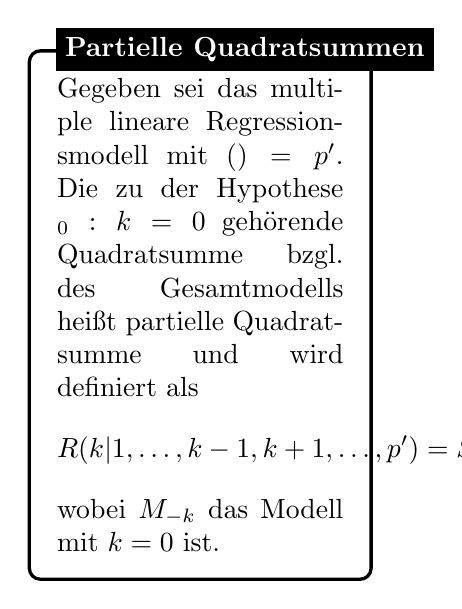
\begin{tikzpicture}
    \node [mybox] (box){%
        \begin{minipage}{0.3\textwidth}
        Gegeben sei das multiple lineare Regressionsmodell mit
        $\rang(\bX) = p'$.
        Die zu der Hypothese $\bH_0: \gb{k} = 0$ gehörende Quadratsumme bzgl.
        des Gesamtmodells heißt \tc{partielle Quadratsumme} und wird
        definiert als
        $$R(\gb{k} | \gb{1}, \dots, \gb{{k-1}}, \gb{{k+1}}, \dots, \gb{{p'}}) = SSE(M_{-k}) - SSE$$
        wobei \tc{$M_{-k}$} das Modell mit $\gb{k} = 0$ ist.
        \end{minipage}
    };
%------------ Partielle Quadratsummen Header ---------------------
\node[fill = black, text=white, font=\bfseries, right=10pt] at (box.north west) 
{Partielle Quadratsummen};
\end{tikzpicture}

%------------ Sequentielle Quadratsummen ---------------
\begin{tikzpicture}
    \node [mybox] (box){%
        \begin{minipage}{0.3\textwidth}
        Gegeben sei das multiple lineare Regressionsmodell mit
        $\rang(\bX) = p'$.
        Wir definieren das Modell \tc{$M_k$} als das Modell
        $$M_k: \bY = \beta_{0} + \beta_{1}\bx + \dots + \beta_{k}\bx_{k} +
        \epsilon$$ Die zu dem Modell $M_k$ gehörende Quadratsumme heißt
        \tc{sequentielle Quadratsumme} und wird definiert als
        $$R(\gb{k} | \gb{0}, \dots, \gb{{k-1}}) = SSE(M_{k-1}) - SSE(M_{{k}})$$ für $k = 1, \dots, p'$.

        Es gilt
        $$SST = \sum_{k=1}^{p'} R(\gb{k} | \gb{0}, \dots, \gb{{k-1}}) + SSE.$$
        \end{minipage}
    };
%------------ Sequentielle Quadratsummen Header ---------------------
\node[fill = black, text=white, font=\bfseries, right=10pt] at (box.north west) 
{Sequentielle Quadratsummen};
\end{tikzpicture}

%------------ R-Code ---------------
\begin{tikzpicture}
    \node [mybox] (box){%
        \begin{minipage}{0.3\textwidth}
        \begin{lstlisting}
# Teste lineare Hypothese der Form 
# H_0: A*beta = c
A <- matrix(c(...))
c <- c(...)
car::linearHypothesis(model, A, c)

# Wenn c =/= 0, dann benutzen wir im 
# model einen offset().

        \end{lstlisting}
        \end{minipage}
    };
%------------ R-Code Header ---------------------
\node[fill = olive, text=white, font=\bfseries, right=10pt] at (box.north west) {R-Code};
\end{tikzpicture}


%------------ Konfidenzellipsoid ---------------
\begin{tikzpicture}
    \node [mybox] (box){%
        \begin{minipage}{0.3\textwidth}
            Gegeben sei das multiple lineare Regressionsmodell mit $\rang(\bX) =
            p'$. Das \tc{Konfidenzellipsoid} für $\bbeta$ zum Niveau $1 - \alpha$ ist gegeben als
            $$\left\{ \bbeta \in \R^{p'} \Big| \frac{1}{p'} (\bbeta - \hbbeta)^\top \hat{\Sigma}_{\hbbeta}^{-1} (\bbeta - \hbbeta) \leq F_{1-\alpha}(p', n-p') \right\}$$
        \end{minipage}
    };
%------------ Konfidenzellipsoid Header ---------------------
\node[fill = black, text=white, font=\bfseries, right=10pt] at (box.north west) 
{Konfidenzellipsoid};
\end{tikzpicture}
    


%------------ Prognosewert ---------------
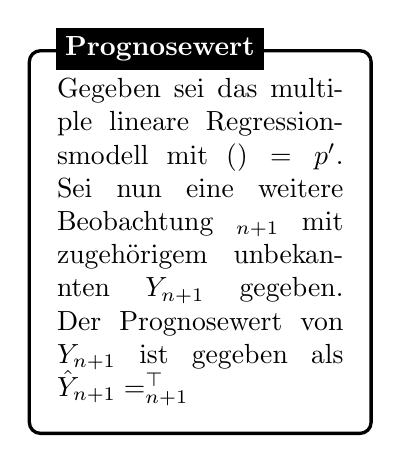
\begin{tikzpicture}
    \node [mybox] (box){%
        \begin{minipage}{0.3\textwidth}
            Gegeben sei das multiple lineare Regressionsmodell mit $\rang(\bX) =
            p'$. Sei nun eine weitere Beobachtung $\bx_{n+1}$ mit zugehörigem
            unbekannten $Y_{n + 1}$ gegeben. Der \tc{Prognosewert von $Y_{n+1}$} ist gegeben als
            $\hat{Y}_{n + 1} = \bx_{n+1}^\top \hbbeta$
        \end{minipage}
    };
%------------ Prognosewert Header ---------------------
\node[fill = black, text=white, font=\bfseries, right=10pt] at (box.north west) 
{Prognosewert};
\end{tikzpicture}
    

%------------ Prognosefehler ---------------
\begin{tikzpicture}
    \node [mybox] (box){%
        \begin{minipage}{0.3\textwidth}
            Gegeben sei das multiple lineare Regressionsmodell mit $\rang(\bX) =
            p'$. Sei nun eine weitere Beobachtung $\bx_{n+1}$ mit zugehörigem
            unbekannten $Y_{n + 1}$ gegeben. Sei $\hat{Y}_{n + 1}$ der Prognosewert. Dann gilt
        \begin{align*}
            \E(\hat{Y}_{n + 1} - Y_{n + 1}) = {} & 0 \\
            \V(\hat{Y}_{n + 1} - Y_{n + 1}) = {} & 
            \ssd \Bigr[ 1 + \bx_{n+1}^\top (\bX^\top \bX)^{-1} \bx_{n+1} \Bigr]
        \end{align*}

        Wir konstruieren das \tc{Prognoseintervall} für $Y_{n+1}$ zum Niveau $1 - \alpha$ als
        $$[\ \hat{Y}_{n+1} - \hat{\sd}_{\hat{Y}_{n+1}}t_{1 - \alpha/2}(n-p');
        \hat{Y}_{n+1} + \hat{\sd}_{\hat{Y}_{n+1}}t_{1 - \alpha/2}(n-p') ]\ $$
        mit
        $$\hat{\sd}_{\hat{Y}_{n+1}} = \hat{\sd}^2 \Bigr[ 1 + \bx_{n+1}^\top (\bX^\top \bX)^{-1} \bx_{n+1} \Bigr].$$

        Wir konstruieren das \tc{Konfidenzintervall} für $\E(Y_{n+1}) = {\mu}_{n+1}$ zum Niveau $1 - \alpha$ als
        $$[\ \hat{Y}_{n+1} - \hssd_{\hat{\mu}_{n+1}} t_{1 - \alpha/2}(n-p'); \hat{Y}_{n+1} + \hssd_{\hat{\mu}_{n+1}} t_{1 - \alpha/2}(n-p') ]\ $$
        mit
        $$\hssd_{\hat{\mu}_{n+1}} = \hssd \Bigr[\bx_{n+1}^\top (\bX^\top \bX)^{-1} \bx_{n+1} \Bigr].$$

        \end{minipage}
    };
    %------------ Prognosefehler Header ---------------------
\node[fill = purple, text=white, font=\bfseries, right=10pt] at (box.north west) 
{Prognosefehler und Prognoseintervall};
\end{tikzpicture}


\end{multicols*}